\chapter{Rationale en doelstelling}\label{ch:introduction}

Sinds de introductie van de \gls{led} is de verlichtingswereld sterk veranderd. In vergelijking met traditionele verlichtingstechnologie\"en zijn \gls{led}s kleine en effici\"ente lichtbronnen. \gls{led}s kunnen verschillende kleuren produceren door basiskleuren te combineren, maar het is moeilijk om effici\"ent kleuren zoals wit te maken. Om dit te bereiken, gebruikt men luminescente materialen zoals fosforen, waarmee men op een effici\"ente manier \gls{led}s in deze kleuren kan cre\"eren. Daarnaast moeten \gls{led}s voldoen aan specifieke kleurweergave-eisen.

Belangrijke begrippen zoals kleur en kleurweergave spelen hierbij een rol. Deze begrippen, de werking van \gls{led}s en de effecten van verschillende factoren zijn echter moeilijk intu\"itief te begrijpen.

Om het aanleren van deze concepten te vergemakkelijken, wordt in deze thesis een educatieve \gls{led} webapp ontwikkeld. In deze app kunnen gebruikers experimenteren met verschillende waarden, \gls{led}s, luminescente materialen, enzovoort, en op een experimentele manier leren over de effecten hiervan.

\section{Bestaande tools}

Er bestaan natuurlijk al tools die vergelijkbare functionaliteiten bieden als die wij in de app willen implementeren. Daarom hebben wij verschillende tools onderzocht en gekeken hoe zij deze functionaliteiten realiseren.

\subsection{Waveform lighting}

Op de website van Waveform Lighting zijn enkele eenvoudige webapps te vinden voor het berekenen van de \gls{spd}, chromaticiteit en de \gls{cri}. Twee van hun beste tools zijn de ``LED Spectrum Simulator'' en de ``Color Rendering Index Calculator''. Deze tools zijn echter op een vrij simpele manier ontworpen. In de spectrum simulator kan de gebruiker bijvoorbeeld alleen het vermogen van vier \gls{led}s met een vast profiel aanpassen. Dit beperkt de mogelijkheid om verschillende combinaties van \gls{led}s uit te proberen en staat dus minder experimentatie toe. De color rendering index calculator biedt wat meer vrijheid, maar is minder gebruiksvriendelijk. De gebruiker moet namelijk alle 401 vermogenswaarden van 380 \gls{nm} tot 780 \gls{nm} handmatig invoeren om de \gls{cri} te berekenen. Bovendien is het bij deze tools minder handig dat deze allemaal apart zijn. Het is dus niet mogelijk om een \gls{spd} te maken en hiervan het effect op chromaticiteit, \gls{cri}, enzovoort te zien. Het zijn echter wel makkelijk te vinden tools die vrij makkelijk te gebruiken zijn. 

\begin{figure}[H]
    \centering
    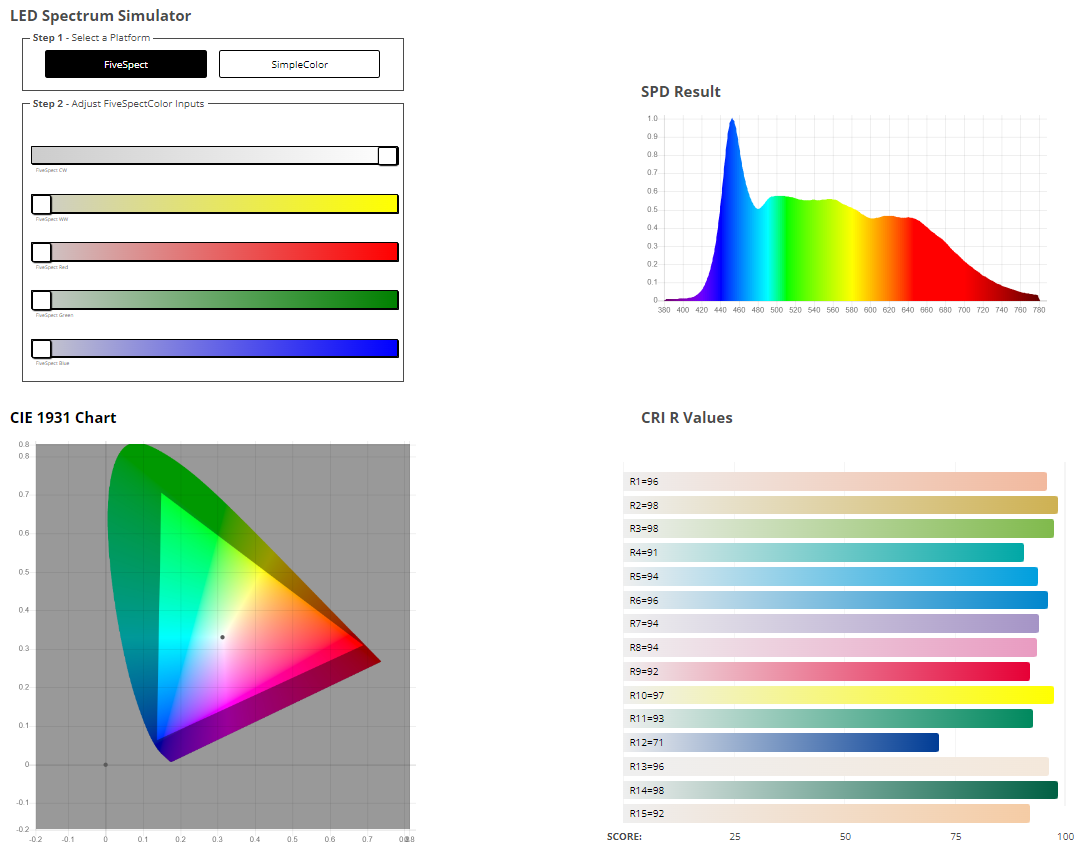
\includegraphics[width=0.95\linewidth]{figs/waveform_spectral.png}
    \caption{Waveform lighting spectrum simulator ~\cite{LEDSpectrumSimulator}}%
    \label{fig:spectrum simulator}
\end{figure}

\subsection{OSRAM ColorCalculator}

De OSRAM ColorCalculator applicatie is een tool die bedoeld is voor het ontwikkelen van ``color mixing \gls{led} lighting solutions''. De software heeft twee hoofdmodi: een ''General photometry'' mode en een ''optimization'' mode. Net als de ''LED Spectrum Simulator'' tool van Waveform Lighting bevat het een chromaticity diagram, \gls{cri}-waarden en een \gls{spd} diagram. Daarnaast biedt het een reeks andere plots, zoals L*a*b*, Delta(u,v), enzovoort. Deze plots zijn echter moeilijker te vinden. Het grootste probleem van de OSRAM ColorCalculator applicatie is echter de drukke \gls{ui}, die de tool moeilijk bruikbaar maakt. Dit zorgt ervoor dat dit een tool is die minder geschikt is voor een lerende gebruiker. Bovendien heeft de applicatie, net als de Waveform Lighting tools, geen mogelijkheid om vrij een \gls{led} toe te voegen met een golflengte tussen 380 nm en 780 nm. Gebruikers moeten \gls{led}s toevoegen met golflengtes in een specifiek bereik. Het grootste probleem is echter dat de applicatie moeilijk te vinden is. Alle downloads op de website van OSRAM zijn verwijderd, en de enige plaats waar de applicatie nog beschikbaar is, is bij de paper op ResearchGate~\cite{selverianColorCalculatorSoftware2017}. Dit maakt het moeilijk voor een gebruiker om de tool te vinden en te gebruiken.

\begin{figure}[H]
    \centering
    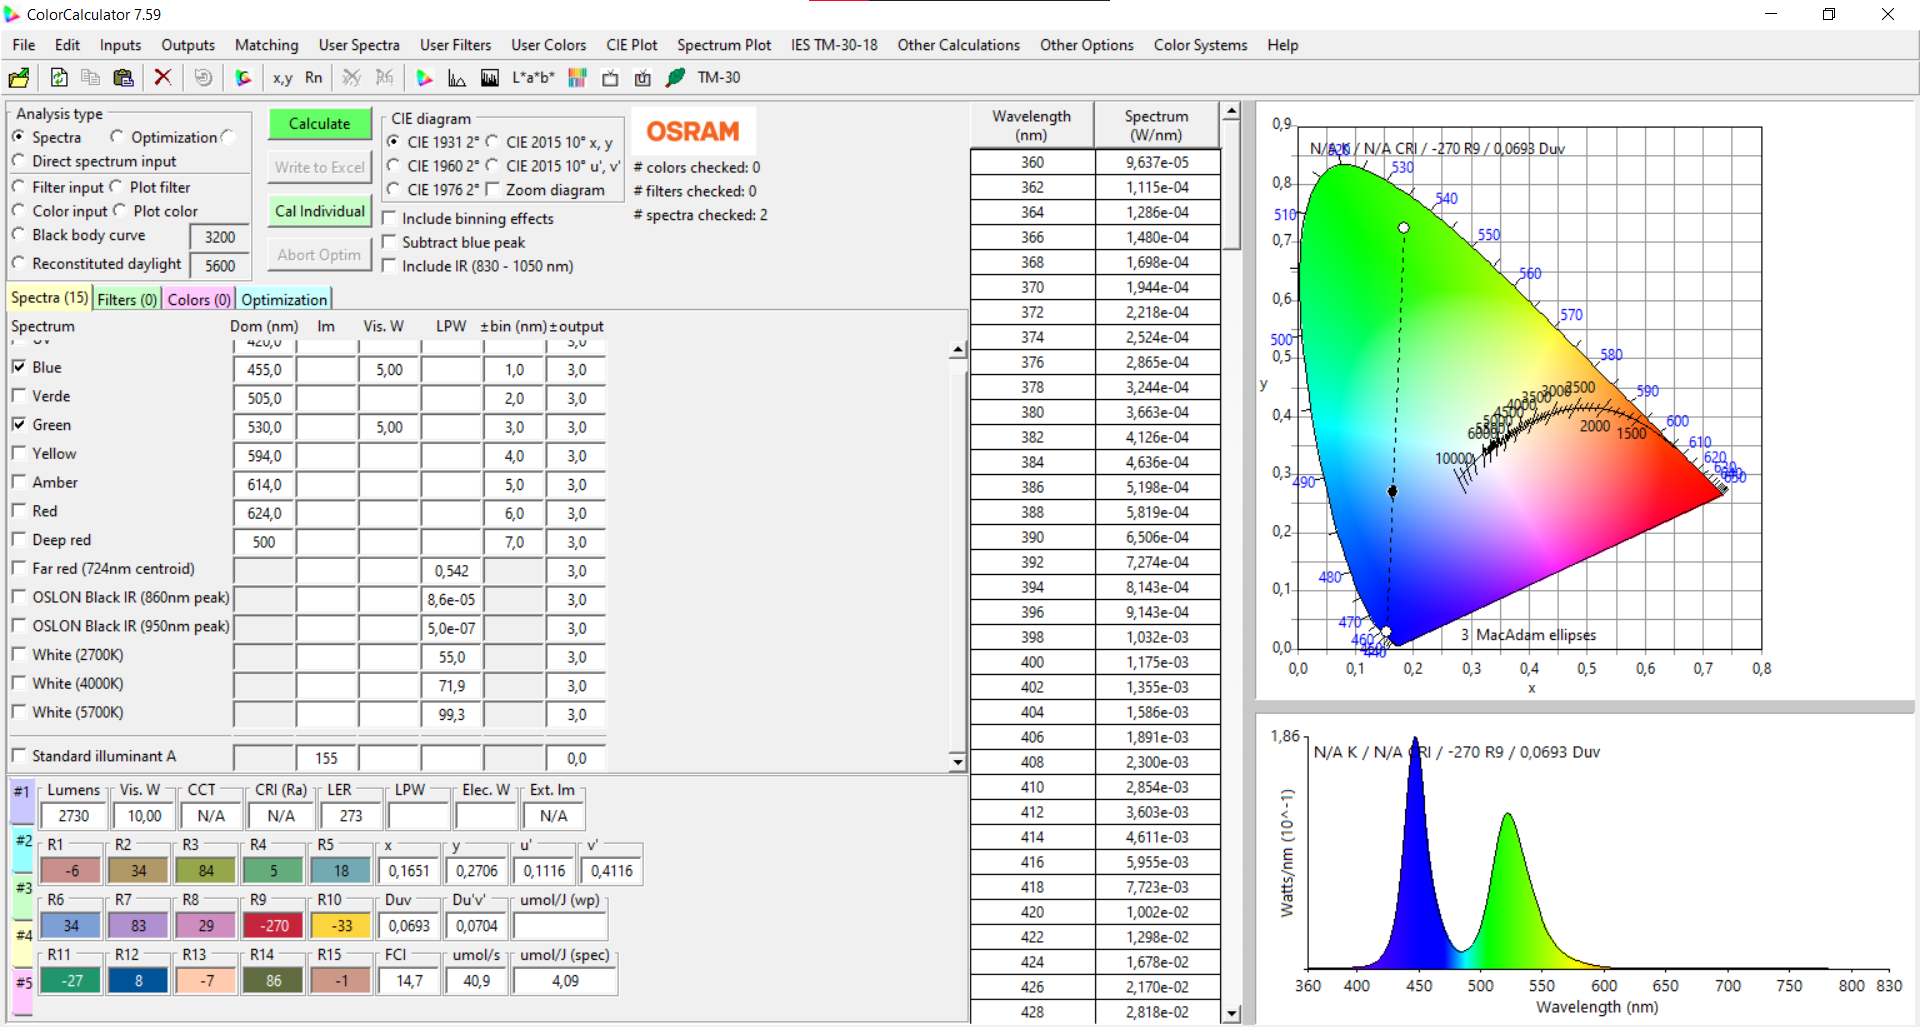
\includegraphics[width=0.95\linewidth]{figs/OSRAM_colorcalculator.png}
    \caption{OSRAM ColorCalculator ~\cite{selverianColorCalculatorSoftware2017}}%
    \label{fig:OSRAM ColorCalculator}
\end{figure}

\subsection{Excel KU Leuven}

Binnen de richting Ingenieurswetenschappen aan KU Leuven Gent wordt een Excel-bestand gebruikt. Dit bestand biedt de mogelijkheid om vier \gls{led}s en twee fosforen in te stellen. Het bevat grafieken van de \gls{spd}, de chromaticiteit, de \gls{eqe} van de \gls{led}s en een color view (met de \gls{cri}). Deze tool is echter niet erg gebruiksvriendelijk, aangezien de gebruiker alle waarden handmatig moet invoeren. Dit maakt het moeilijk voor de gebruiker om met waarden te experimenteren en de effecten daarvan te zien. Bovendien wordt experimenteren bemoeilijkt doordat de resultaten en de inputs zich op verschillende tabbladen bevinden. Ten slotte is deze Excel alleen beschikbaar voor studenten van KU Leuven die het vak volgen waarin deze wordt gebruikt.

\subsection{Conclusie}

Er zijn dus al enkele tools beschikbaar die vergelijkbare functionaliteiten bieden. Deze tools zijn echter te simpel, te ongebruiksvriendelijk en moeilijk te vinden. Bovendien zijn er geen tools die functionaliteit voor luminescente materialen zoals fosforen en quantum dots aanbieden. Het is dus zeker een goed idee om een gebruiksvriendelijke, gemakkelijk te vinden webapp te ontwikkelen die deze functionaliteiten implementeert. De grootste voordelen van onze webapp zijn dus de vrijheid van gebruik en de simulatie van luminescente materialen. Daarnaast bied de app een grotere mogelijkheid tot experimenteren.





